Um ein zu verifizierendes GALS-Modell vollständig zu definieren müssen die folgenden Eigenschaften spezifiziert werden:
\begin{itemize}
\item Die synchronen Komponenten, aus denen das Gesamtsystem zusammen gesetzt wird.
  Jede synchrone Komponente ist eine Instanz eines in einer synchronen Sprache spezifizierten Modells.
\item Die Verbindungen zwischen den Komponenten.
  Eine Verbindung verknüpft eine Ausgabevariable einer Komponente mit einer Eingabevariable einer anderen.
\item Die zu verifizierende Eigenschaft in Form einer LTL Formel über die Variablen der einzelnen Komponenten.
\end{itemize}

Die GTL-Sprache verwendet externe Formalismen, um die synchronen Komponenten zu beschreiben.
Auf die Implementierungen der synchronen Komponenten wird in der Beschreibung nur verwiesen.
Hierfür wird das Schlüsselwort \emph{model} verwendet.
Das folgende Codefragment deklariert eine Komponente mit dem Namen \emph{EntrySensor}, die im \emph{SCADE}-Formalismus definiert wurde:
\begin{lstlisting}[language=gtl]
  model[scade] EntrySensor("LightBarrier");
\end{lstlisting}
Die Ausdrücke in Klammern ("`LightBarrier"') machen formalismus-spezifische Angaben, in diesem Fall geben sie beispielsweise die Klasse des gewünschten Modells an.
Zu beachten ist, dass in der Komponentendeklaration keine Ein- oder Ausgabekanäle definiert werden.
Die GTL-Sprache setzt voraus, dass diese implizit in dem Modell-Formalismus vorhanden sind.

Um nun Zusicherungen zu formulieren, die die Komponente einhalten wird, kann man die Deklaration um so genannte Kontrakte erweitern:
\begin{lstlisting}[language=gtl]
  model[scade] EntrySensor("LightBarrier") {
    obscured and (next obscured) and (not offline) => alert;
  }
\end{lstlisting}
Dieser Kontrakt besagt beispielsweise, dass wenn der Sensor der Lichtschranke zwei Zeitschritte verdeckt ist und der Sensor nicht ausgeschaltet ist, auf jeden Fall Alarm ausgelöst wird.
Kontrakte dürfen nur Aussagen über Variablen der lokalen Komponente machen.

Die Verbindungen zwischen Komponenten werden durch \emph{connect}-Deklarationen angegeben.
Eine Verbindung gibt dabei eine Variable einer Komponente an, von der sie ausgeht und eine Variable eines anderen Modells, zu der sie geht.
\begin{lstlisting}[language=gtl]
  connect EntrySensor.alert TrapDoor.open;
\end{lstlisting}
Diese Verbindung gibt beispielsweise an, dass das Ausgabesignal \emph{alert} der Komponente \emph{EntrySensor} mit dem Eingabesignal \emph{open} der Komponente \emph{TrapDoor} verbunden sein soll.
Es können nur Ausgabesignale mit Eingabesignalen verknüpft werden.

Um nun Aussagen über das Gesamtsystem treffen zu können, verwendet man das \emph{verify}-Schlüsselwort.
Mit diesem lassen sich LTL-Formeln angeben, die Gültigkeit im System besitzen sollen.
\begin{lstlisting}[language=gtl]
  verify {
    always (System.offline => not TrapDoor.open);
  }
\end{lstlisting}
Im Gegensatz zu Kontrakten können diese Formeln Variablen aus mehreren Modellen enthalten.
Die gesamte Grammatik der GTL-Sprache ist in Abbildung \ref{fig:grammar} angegeben.

\begin{figure}
  \centering
  \begin{grammar}
    <declaration> ::= `model' `[' <id> `]' <id> `(' (<argument> (`,' <argument>)*)? `)' <model\_contract>
    \alt `connect' <id> `.' <id> <id> `.' <id> `;'
    \alt `verify' `{' (<formula> `;')* `}'
    
    <model\_contract> ::= `{' (<formula> `;')* `}'
    \alt `;'
    
    <formula> ::= <var>
    \alt <lit> `<' <lit>
    \alt <lit> `>' <lit>
    \alt <lit> `<=' <lit>
    \alt <lit> `>=' <lit>
    \alt <lit> `=' <lit>
    \alt <id> `in' `{' (<lit> (`,' <lit>)*)? `}'
    \alt `not' <formula>
    \alt <formula> `and' <formula>
    \alt <formula> `or' <formula>
    \alt <formula> `follows' <formula>
    \alt `always' <formula>
    \alt `next' <formula>
    \alt `(' <formula> `)'
    
    <lit> ::= <int>
    \alt <var>
    
    <var> ::= <id>
    \alt <id> `.' <id>

    <id> ::= (`a'-`z' `A'-`Z' `0'-`9')+
    
    <int> ::= (`0'-`9')+
  \end{grammar}
  \caption{GTL Grammatik}
  \label{fig:grammar}
\end{figure}

\section{Formeln}
Die Ausdrücke, die zur Spezifikation von Kontrakten sowie zur Formulierung von einzuhaltenden Bedingungen verwendet werden, stellen eine Untermenge der so genannten LTL-Formeln (LTL steht für "`linear temporal logic"') dar.
Da der SCADE Design Verifier nicht in der Lage ist, Liveness-Eigenschaften zu verifizieren, können in den Formeln allerdings keine \emph{until}-Konstrukte verwendet werden.

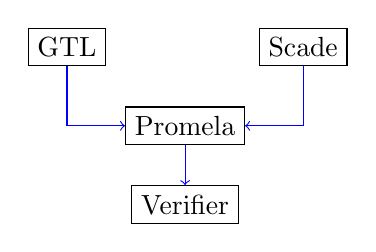
\begin{tikzpicture}
  \node[draw] (promela) at (1.5,1) {Promela};
  \node[draw] (gtl) at (0,2) {GTL};
  \node[draw] (scade) at (3,2) {Scade};
  \node[draw] (verifier) at (1.5,0) {Verifier};
  \draw[->,blue] (scade) |- (promela);
  \draw[->,blue] (gtl) |- (promela);
  \draw[->,blue] (promela) -- (verifier);
\end{tikzpicture}

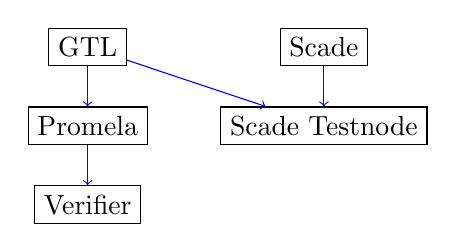
\begin{tikzpicture}
  \node[draw] (gtl) at (0,2) {GTL};
  \node[draw] (scade) at (3,2) {Scade};
  \node[draw] (promela) at (0,1) {Promela};
  \node[draw] (testnode) at (3,1) {Scade Testnode};
  \node[draw] (verifier) at (0,0) {Verifier};
  \draw[->,blue] (gtl) -- (promela);
  \draw[->,blue] (scade) -- (testnode);
  \draw[->,blue] (gtl) -- (testnode);
  \draw[->,blue] (promela) -- (verifier);
\end{tikzpicture}

